\documentclass[12pt, a4paper]{article}

%los use packages van aquí
\usepackage[english]{babel}
\usepackage[utf8]{inputenc}
\usepackage{amsfonts}
\usepackage{amsmath}
\usepackage{amssymb}
\usepackage{tabularx}
\usepackage{listings}
\usepackage{graphicx}
\usepackage[dvipsnames]{xcolor}
\usepackage{setspace}
\usepackage[left=2.54cm, right=2.54cm, top=2.54cm, bottom=2.54cm]{geometry}
\usepackage{xcolor}
\usepackage{float}
\usepackage{hyperref}

\definecolor{backcolour}{rgb}{0.95,0.95,0.92}
\definecolor{codegreen}{rgb}{0,0.6,0}

\lstdefinestyle{mystyle}{
	backgroundcolor=\color{backcolour},   
	commentstyle=\color{gray},
	keywordstyle=\color{codegreen},
	numberstyle=\tiny\color{codegreen},
	stringstyle=\color{magenta},
	basicstyle= \ttfamily,
	breakatwhitespace=false,         
	breaklines=true,                 
	captionpos=b,                    
	keepspaces=true,                                   
	showspaces=false,                
	showstringspaces=false,
	showtabs=false,                  
	tabsize=2,
	numbers=left
}

\lstset{style=mystyle}

\setlength{\parindent}{1em}
\setlength{\parskip}{1em}
\renewcommand{\arraystretch}{1.5}

\title{Exploration of Parkinson's disease recognition space by artificial neuron networks.}
\author{Mario Rojo Vicente}
\date{}	 							%fecha de entrega

\addto\captionsenglish{\renewcommand*\contentsname{\LARGE Summary}} %cambia nombre del índice

\begin{document}
	
	 \begin{titlepage}
	\begin{center}
		{\huge \textbf{Technical University of Madrid}}\\
		\vspace{5mm}
		{\large \textbf{Engineering the future}}\\
		\vspace{5mm}
		\begin{figure}[h]
			\centering
			
\includegraphics[height = 8cm]{img/insigneaUPM.jpg}
		\end{figure}
		\vspace{5mm}
		{\LARGE \textbf{Computer Systems Department}}\\
		\vspace{5mm}
		{\large \text{Higher Technical School of Computer Systems Engineering}}\\
		\vspace{5mm}
		\textcolor{RoyalBlue}{\rule{\linewidth}{0.75mm}}\\
		\vspace{2mm}
		\begin{spacing}{1.5} %solo si el título tiene más de una linea
			{\Large \textsc{Exploration of Parkinson's disease recognition space by artificial neural networks.}}
		\end{spacing}
		\textcolor{RoyalBlue}{\rule{\linewidth}{0.75mm}}\\
		\vspace{1cm}
		{\Large \text{Writen by:}}\\
		\vspace{5mm}
		{\Large \textbf{Mario Rojo Vicente}}\\
		\vspace{5mm}
		{\Large \text{Directed by:}}\\
		\vspace{5mm}
		{\Large \textbf{Francisco Díaz Pérez}}\\
		\vspace{5mm}
		{\Large \text{Bachelor Thesis for the Software Engineering Degree}}\\
		\vspace{5mm}
		{\Huge \textbf{June 2022}}
	\end{center}
\end{titlepage}
	
	\section*{}
	\begin{flushright}
		\vspace*{\fill}
		Acknowledgment
		\vspace*{\fill}
		
	\end{flushright}

	\clearpage
	
	\section*{Abstract}
	
	%purpose, method, scope, results, and conclusion
	
	\clearpage
	
	\tableofcontents
	
	\clearpage
		
	\section{Introduction}
	
	\subsection{Context}
	
	The origin of Parkinson´s disease is at best unclear. While some authors claim it to be a consequence of unknown toxins introduces in the XIX century during the Industrial Revolution, many historical evidences suggest that the presence of this ailment goes as far back as the 2000-1500 ac, when some of its symptoms where first references in the Vedas texts. Further references to what could possibly be Parkinson´s disease were also found in Egyptian papyrus and ancient Chinese medical treaties, among other historical documents. Also, several historical personalities, such as Hipocrates, an ancient Greek´s doctor, and the Italian genius Leonardo Da Vinci, analyzed and studied several symptoms related to this illness.
	
	The first publication referencing what we currently know as Parkinson´s disease was a paper by the name "An essay on the shaking palsy", published in 1817 by the British surgeon James Parkinson. None the less, the disease did not get its final name until the year 1880 when Jean-Marie Charcot, a well recognized french neurologist that was researching the stiffness related to the shaking palsy, proposed to rename the disease in honor of his English colleague.\cite{parkinsonhistoria}
		
	In "An essay on the shaking palsy" James Parkinson referred to the shaking palsy as an "Involuntary tremulous motion, with lessened muscular power, in parts not in action and even when supported; with a propensity to bend the trunk forwards, and to pass from a walking to a running pace: the senses and intellects being uninjured"\cite{parkinson2002essay}. Nowadays the definition for Parkinson´s disease establishes it as a progressive multi-system neurodegenerative disorder more common among people in later years of live, and several studies refer to it as the second most common neurodegenerative illness worldwide.\cite{sveinbjornsdottir2016clinical}
	
	In modern medicine it is a common practice among physicians to refer to the mnemonic TRAP (Tremor, Rigidity, Akinesia and Postural Instability) when diagnosing the Parkinson´s disease, which includes definitions for all it´s main clinical features. Even though nowadays Parkinson´s disease is far more established and recognized, it´s correct and early diagnosis still represents a challenge as many of its signs and symptoms are often insidious. Even when referring to the TRAP, many of its symptoms can only be identified through some sort of examination that will normally not be considered unless specifically looking for those. Some of the symptoms of Parkinson´s disease that are easier to detect are the following:\cite{frank2006approach}
	
	\begin{itemize}
		
		\item The Gait of patients with Parkinson´s disease. Which is characterized for the forward flexion of the trunk and a decrease in the length and height of step. This characteristics can be noticed even before the appearance of the postural instability, but can easily be confused with the symptoms of the senile gait related to the aging process.
		
		\item The development of a masklike face, also known as hypomimia, which is composed of two main factors. A decrease in the blink frequency of the patient and an increased dabbing or drooling due to the difficulty of swallowing saliva that patients of Parkinson´s disease and other parkinsonian illnesses experiment.
		
		\item The development of micrography, which can be identified by a doctor observing a patient do a written task or even by the sufferer himself.
		
		\item The suffering of depression, which is the most common psychiatric feature present in the early stages of the Parkinson´s disease.
		
		\item The development of dementia which is more of a complication common in  the later stages of Parkinson´s disease.
		
	\end{itemize}
		
	When taking about Parkinson´s disease we must realize that it´s early detection has a mayor impact on the ability to control it´s development. Nowadays, newer means of technology allow for newer approaches regarding the diagnosis of Parkinson´s disease, and so many later papers focus on the possibility of relying on Artificial Intelligence and Machine Learning to establish patterns based on the parametrization of different data related but not limited to aspects such as the phonic and kinematic disorders that are attributed to this illness. 
	
	
	
	

	\clearpage
		
	\subsection{Objective}
	
	The main objective is this paper is to implement a convolutional neuronal network based system for the early detection of Parkinson´s Disease based on the parametrization of audio recordings. In order to do so I will based my research on data taken out from Synapseg.
	
	This objective can be therefore subdivided in the following:
	
	\begin{enumerate}

		\item Get familiarized with the Python programming language and the Jupiter Notebook environment.
		
		\item Learn the possibilities offered by python´s deep learning API keras.
		
		\item Research the state of art concerning both the possible structures for Neuronal Networks that could be relevant for this project, as well as previous researches on this topic.
		
		\item Analyze the raw audio data in order to extract the relevant information to then feed into the Neuronal Networks.
		
		\item Implement, train and compare the results of different Neuronal Network´s architectures, in order to provide evidence of their effectiveness regarding the early detection of Parkinson´s Disease based on the provided information.
		
		\item Draw conclusions based on the results of the experiments and provide this information so further research can be realized if the results end up been encouraging.
		
	\end{enumerate}

	To facilitate this projects success I will also establish the following "Machine Learning Project Checklist" as suggested by Aurélien Géron in his book "Hands-On Machine Learning with Scikit-Learn, Keras, and TensorFlow" \cite{handsonmachinelearning}:
	
	 \begin{enumerate}
	 	\item Frame the problem and look at the big picture.
	 	
	 	\item Get the data.
	 	
	 	\item Explore the data to gain insights.
	 	
	 	\item Prepare the data to better expose the underlying data patterns to Machine Learning algorithms.
	 	
	 	\item Explore many different models and shortlist the best ones.
	 	
	 	\item Fine-tune your models and combine them into a great solution.
	 	
	 	\item Present your solution.
	 \end{enumerate}
	
	
	\clearpage
	
	\subsection{Document Structure}
	
	Following this introduction the paper will be structured according to the following sections:
	
	\begin{itemize}
		
		\item \textbf{State Of Art:}
		
		\item \textbf{Theoretical Bases:}   
		
		\item \textbf{Data:}
		
		\item \textbf{Conclusion:}
		
		\item \textbf{Social Implications:}
		
	\end{itemize}

	\clearpage
	
	\subsection{State Of Art}
	
	When regarding the application of machine learning techniques to the diagnosis of Parkinson´s disease there is a wide range of papers that each present their personal take on the matter.
	
	There are several concerns that need to be addressed when approaching this issue from a technological perspective, the first of which would be to decide on the type of data that is going to be fed into the algorithm.
	
	While some papers focus on the parametrization of the speech, such as "Diagnosis of Parkinson's disease using deep learning and cell phone voice recordings" \cite{deeplearningygrabaciones} others choose to analysis different sources of data that they feel could present interesting patterns. One possibility would be to realize a kinematic analysis of the patient, using data describing motion of upper and lower extremities, as implemented in "Artificial intelligence for assisting diagnostics and assessment of Parkinson’s disease—A review" \cite{belic2019artificial}, while several studies in the platform Synapse investigate the possibility of diagnosing Parkinson´s Disease through symptoms related to the loss of recent memory as well as the study of the patients manual abilities.
	
	When choosing the data to be sampled for the experiments it is also relevant to consider the pros and cons of selecting numerous sources of data versus choosing to focus on one specific type. For this paper I have decided to focus on studying voice recordings exclusively, as I find those to have great potential. Nonetheless, I will try to identify any possible relations between the outcomes of the machine learning algorithms application, and other data concerning the state of the patients such as several measurements related to the Unified Parkinson's Disease Rating Scale (UPDRS). The idea of utilizing speech analysis to detect and track the deterioration associated to the evolution of the disease comes from sysmtoms such as Dysarthria that affect this functions. \cite{cnntoformantmeasures}
	
	After choosing the data, it needs to be analyzed in order to separate all the relevant information from the useless bits and noise, for that we will focus on analyzing sets of traits for the data that have previously proven good efficacy when utilizing IA and Deep learning. This will be later discussed on the \hyperref[sec:Data]{\textbf{Data}} section of this document.
	
	The last thing to do would then be to choose a Neuronal Network architecture to implement, but this will be furthered discussed in the following \hyperref[sec:TheoreticalBases]{\textbf{Theoretical Bases}} section.
	
	\clearpage
	
	\section{Theoretical Bases}
	\label{sec:TheoreticalBases}
	
	In this paper we will be working within the field of Machine Learning, so in order to describe it I will refer to Tom Mitchell, who once described Machine Learning as: 
	
	\textit{"A computer program is said to learn from experience E with respect to some task T and some performance measure P, if its performance on T, as measured by P, improves with experience E."}
	\begin{flushright}
		\textit{- Tom Mitchell, 1997 \cite{handsonmachinelearning}}
	\end{flushright}
	
	Within the context of Machine Learning there exits the branch of Deep Learning, which focuses on training Deep Neuronal Networks, this been stacks of artificial neurons that aim to represent, in a very simplified way, the human´s cerebral cortex. Which is relevant because as I will explain on the following subsection I have decided to implement a Convolutional Neuronal Network (CNN) which happens to be one of the main algorithms that belong to this category of machine learning.
	
	%Applying ML techniques to dig into large amounts of data can help discover patterns that were not immediately apparent. This is called data mining.
	
	\clearpage
	
	\subsection{Types of Machine Learning Systems }
	
	When working with Machine Learning Systems (MLS) there are several questions that have to be answered in order to decide what type of systems best fits the problem at hand: \cite{handsonmachinelearning}
	
	\begin{itemize}
		
		\item Will the system be trained with or without human supervision ?
		
		\item Will the system be able to learn incrementally on the fly ?
		
		\item Will the system be able to detect patterns and build predictive models ?
		
	\end{itemize}
	
	The answer to the first question will allow as to find which of the following four categories of MLSs best suits our model according to the amount and type of supervision they get during their training process: 
	
	\begin{itemize}
	
	\item \textbf{Supervised Learning:} in this type of training the data used for this purpose is accompanied by the desired outcomes of the system for every data instance to be used as input, those outcomes are often referred to as labels. This category includes machine learning algorithms such as Decision Trees and Support Vector Machines.
	
	\item \textbf{Unsupervised Learning:} in this case the train data set provided to the algorithm it´s fully unlabeled. This category includes machine learning algorithms such as clustering and association rule learning.
	
	\item \textbf{Semisupervised Learning:} as its name suggests, semisupoervised learning is a method that is half way between supervised and unsupervised learning and is most useful when working with partially labeled data sets. This category includes machine learning algorithms such as deep belief networks. The algorithms included in this group are often constructed by combining supervised and unsupervised algorithms.
	
	\item \textbf{Reinforcement Learning:} in this case the MLS, often referred to as agent within this context, will analyze its environment, chose and perform actions and then receive a reward or penalty as a consequence of its interaction with the environment. Some examples of machine learning algorithms that fall within this group are DeepMind’s AlphaGo and many robot´s walking algorithms. 
	
	\end{itemize}

	Following the first, the second question will allows us to differentiate between the following two different groups of algorithms:
	
	\begin{itemize}
	
	\item \textbf{Batch Learning:} that encompasses those algorithms that need to be trained before been released to the public, using all the available data and that will not learn once deployed. This type of training often requires a big amount of resources and time to train and it requires to train and deploy a new stance of the product every time we wish for the MLS to take into account any new data.
	
	\item \textbf{Online Learning:} which includes all the algorithms that have the particularity of been able to learn after their deployment. This group is trained by sequentially feeding it with instances of the data that could be organized in small groups, often called mini batches, or individually. Due to its characteristics the algorithms within this group are often implemented in applications that require a rapid and autonomous adaptation to new incoming data or those that aim to run using limited computing resources.
		
	\end{itemize}
	
	
	Finally the last and third question will help us differentiate between:
	
	\begin{itemize}
		
	\item \textbf{Instance-based learning:} this group focuses on learning all data within the training set by heart and then implementing a measures that establishes the similarity of the new instance to the ones used for training and generalizes based on this measure so it can predict its corresponding outcome.
	
	\item \textbf{Model-based learning:} which instead of predicting the outcomes by learning the training examples uses a model chosen by the architect of the MLS. The architect will often choose a model based on an analysis of the data related to the problem ans their own expertise.
		
	\end{itemize}

	For this paper I plan on implementing a MLS that I will train personally with a fully labeled dataset, that will not be required to learn incrementally on the fly but rather will be trained once and then analyzed and that will work based on intances due to the complexity of the data. It is also relevant to consider that in this case we will be analyzing parameterized audio recordings and that is why I considered it could be interesting to try and implement one of the systems that work best for voice recognition, which I found to be RNNs (Recursive Neuronal Networks), CNNs (Convolutional Neuronal Networks) and Transformers.
	
	Taking all the characteristics from both the project and the dataset into account, as well as the fact that I will be working with audio recordings, I decided that the best MLS for this paper would be a Convolutional Neuronal Network (CNN).
	
	\clearpage
	
	\subsection{The CNN Model and VGG Architecture}
	
	In order to understand what a CNN is, we first need to establish a definition for Neuronal Network. 
	
	Therefore we will establish an Artificial Neuronal Network (ANN) also referred to as Neuronal Network (NN) to be a machine learning model based of the networks of biological neurons found in our brains. This model is constituted by one or more layers of any number of artificial neurons, which are at the same time inspired in their biological counterpart. While the original model came from this biological analogy, with time ANN have deviated further and further away from their biological counterpart and so today some researchers argue that this analogy should no longer be considered appropriate.
	
	Now that we have a basic understanding of what a ANN is be can further delve into our solution by addressing what a CNN truly is and what makes them stand out from other ANN based models.
	
	On 1958\cite{cortex58} and 1959\cite{cortex59} David H. Hubel and Torsten Wiesel, realized several experiments on the structure and working mechanics of the visual cortex of cats. This studies set the foundations of the biological model that later on will serve as analogy for the creation of the Neocognitron\cite{neocognitron} in 1980 which was the predecessor of the more modern CNNs.
	
	CNN architectures are often constructed with several building blocks common to other Neuronal Networks such as \textit{Fully Connected Layers}\footnote{A fully connected layer is a type of layer in which all its neurons are all connected to every element of the input of the layer.} and \textit{Sigmoid Activation Functions}\footnote{The sigmoid function is given by $\sigma(x) = 1/(1+exp(-x))$.}\footnote{An activation function is a function implemented by some artificial neurons to produce its output given a weighted sum of inputs. There are many type of activation functions such as sigmoid and relu. }, but also include two more specialized building blocks the Convolutional and Pooling layers:
	
	\begin{itemize}
		
		\item \textbf{Convolutional Layer:} this new type of layer works by connecting its neurons not the totality of the output of the previous layer, but rather to a smaller rectangular fraction of it, referred to as the neuron´s receptive field. In an image for example a particular neuron could be connected to a grid of $Z \cdot Y$ adjacent pixels. 
		
		\begin{figure}[H]
			\centering
			\label{ConvLayer}
			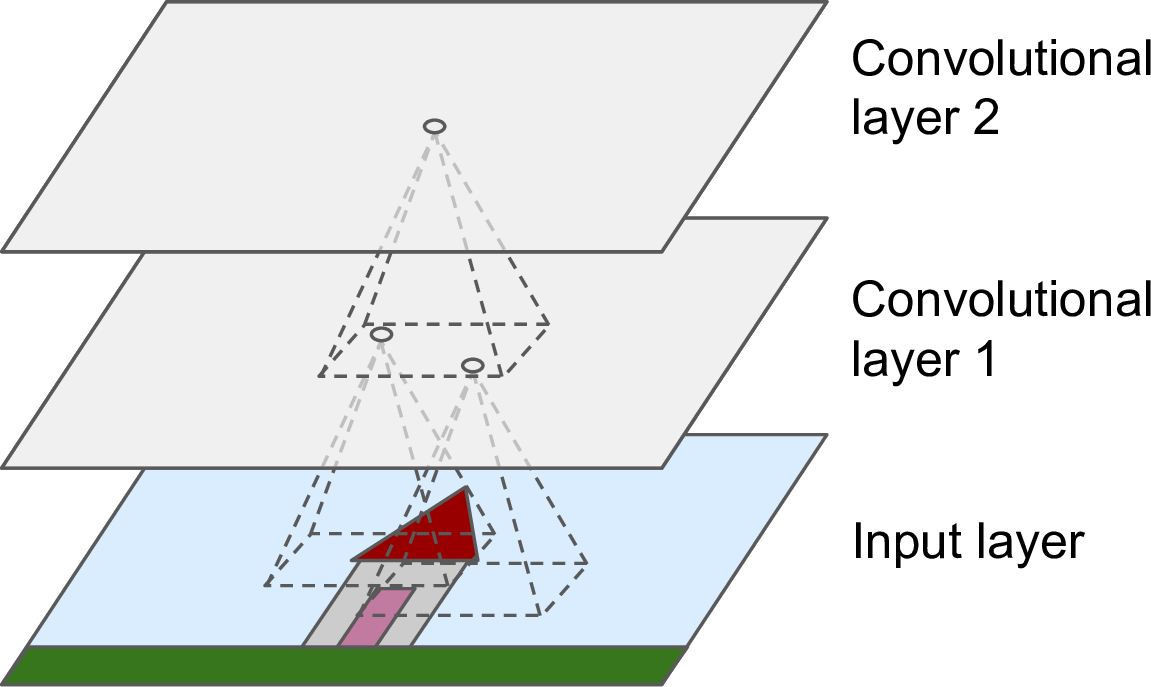
\includegraphics[height=38mm]{img/convLayer.png}
			\caption{Visual representation of the effects of convolution layers.\cite{handsonmachinelearning}}
		\end{figure}
		
		\item \textbf{Pooling Layer:} this layer is often used to reduce the risk of overfitting as well as the computational requirements of any CNN. It works much like the previously described convolutional layer, its objective been to subsample the layer´s input. In this layer the artificial neurons apply an aggregation function such as the max or mean to their input in order to reduce its dimensions,
		
	\end{itemize}
	
	\begin{figure}[H]
		\centering
		\label{MaxPoolLayer}
		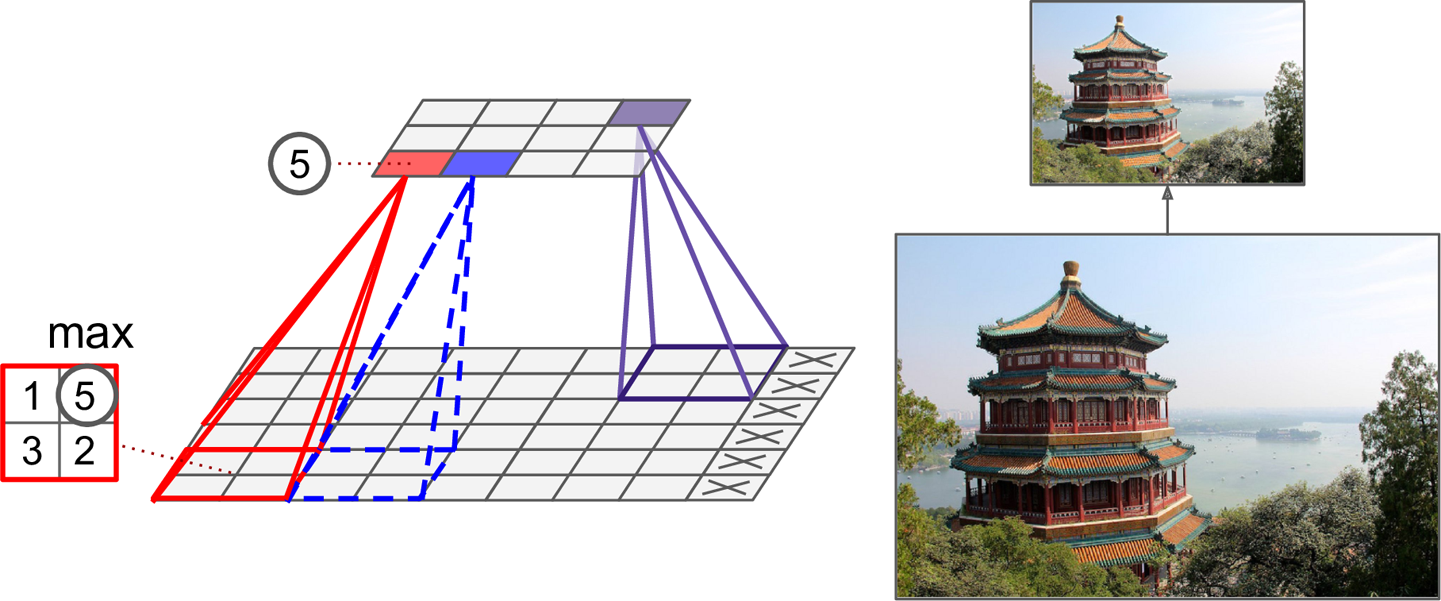
\includegraphics{img/maxPoolingLayer.png}
		\caption{Visual representation of the effects of pooling layers. \cite{handsonmachinelearning}}
	\end{figure}

	After realizing extensive research and discussing with several peers and professors I decided to go with the Visual Geometry Group (VGG) architecture for my neuronal network which focuses on the use of deep convolutional models. Based on this architecture two main models have been established that are referred to by the architecture´s acronym followed by the number of layers they support, those been the VGG-16 and VGG-19 models.\cite{VGGinfo}
	
	\vspace{5mm}
	\begin{figure}[h]
		\label{VGGArchitecture}
		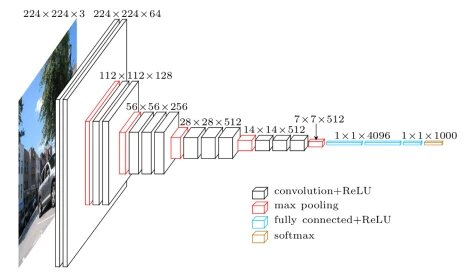
\includegraphics[width=150mm]{img/vgg-neural-network-architecture.jpg}
		\caption{Visual representation of a VGG architecture. \cite{VGGimg}}
	\end{figure}
	\vspace{5mm}

	From the two models previously presented I decided to apply in this paper the VGG-16 architecture, the smaller of the two, as the problem at hand only has a dimensionality of 40 (there are 40 attributes that will be imputed in the network), and if the models turns out to be too big for the problem it could lead to problems such as overfitting. This will be furthered developed in the subsection \hyperref[sec:ProblemsWithAlgorithm]{\textbf{Problems with the Algorithm}} of the \hyperref[sec:CNNImplementation]{\textbf{Implementation of the CNN}} section of this paper.
	
	
	\clearpage
	
	\section{Data}
	\label{sec:Data}
	
	In order to apply any Machine Learning algorithm we need a data set, in this case I will be utilizing one extracted from the Synapse platform. This data set provides 74 different data from a total of 779 participants, all of which has been previously anonymized. From the initial data I will only feed values for the following 40 attributes to the Neuronal Network:
	
	\vspace{5mm}
	
	%
\begin{tabularx}{1\textwidth} { 
		| >{\raggedright\arraybackslash}X 
		| >{\raggedright\arraybackslash}X 
		| >{\raggedright\arraybackslash}X 
		| >{\raggedright\arraybackslash}X |}
	\hline
	\textbf{Name} & \textbf{Description} & \textbf{Type} & \textbf{Units} \\
	\hline
	feature01  & Median F0  & real & Hz  \\
	\hline
	feature02  & Mean absolute F0 time derivative  & real & Hz^2 \\
	\hline
	feature03  & Median absolute F0 time derivative  & real & Hz^2  \\
	\hline
	feature04  & Mean absolute value of time derivative of RMS power  & real & Hz  \\
	\hline
	feature5  &Median absolute value of time derivative of RMS power  & real & Hz  \\
	\hline
	feature06-feature19  & Median cepstral coefficients 0-12 for entire voice recording  & real & None  \\
	\hline
	feature20-feature32  & Mean absolute time derivative of cepstral coefficients 0-12 across entire voice recording  & real & None  \\
	\hline
	feature33  & Recurrence period density entropy (RPDE) Hnorm  & real & None  \\
	\hline
	feature34  & Detrended fluctuation analysis (DFA) scaling parameter alpha  & real & None  \\
	\hline
	feature35  & Modified pitch period entropy (PPE)  & real & None  \\
	\hline
	feature36  & Relative spectral power 0-500Hz  & real & None  \\
	\hline
\end{tabularx}

\begin{tabularx}{1\textwidth} { 
		| >{\raggedright\arraybackslash}X 
		| >{\raggedright\arraybackslash}X 
		| >{\raggedright\arraybackslash}X 
		| >{\raggedright\arraybackslash}X |}
	\hline
	feature37  & Relative spectral power 500-1kHz  & real & None  \\
	\hline
	feature38  & Relative spectral power 1kHz-2kHz  & real & None  \\
	\hline
	feature39  & Relative spectral power 2kHz-4kHz  & real & None  \\
	\hline
	current\_age  & Age of participant when call was recorded  & Integer & Years  \\
	\hline
	sex  & Sex of participant  & String & ‘M’/’F’/empty  \\
	\hline
\end{tabularx}


	
	\vspace{5mm}
	
	I have selected all the parameters related to the voice recordings as well as the sex and current age which I believe could be relevant for the classification process.
	 
	Some of the data from the data set that will not be fed to the Neuronal Network relates to the previously mentioned UPDRS (Unified Parkinson's Disease Rating Scale) and will be utilized later on in order to draw any possible relations between those and the outcomes of the Neuronal network. As this data is not directly related to the voice recordings I have not considered it relevant for the inputs of the Neuronal network which affects the gradient.
	
	Previous to its use in the training and validation of the Neuronal Network the data set must be load and go through several processes. In order to load the data I will use python´s Pandas library, which will allow me to generate panda´s data frames from the original coma separated CSV files.
	
	\clearpage
	
	\subsection{Cleaning The Data Set }
	
	The process of cleaning the data will prevent the Neuronal Network from learning any incorrect patterns that may arise of such data and it makes the process of learning more efficient as the incorrect instances would slow down the learning process pushing the weights and bias in wrong directions.
	
	I started the data cleaning process by simply removing all the instances for which the attribute "voice\_code", which can take the values "ok" or "bad", had de "bad" value, as those do not include any values for any of the "features" which are to be imputed in the Neuronal Network. To do so I implemented the following function:
	
	\vspace{5mm}
	
	\begin{lstlisting}[language=Python]
		
	def eliminateBadVoiceCodeElements(data_frame):
			valid_voice_code_elemnts = data_frame.copy()
			valid_voice_code_elemnts = valid_voice_code_elemnts.drop(valid_voice_code_elemnts[valid_voice_code_elemnts["voice_code"] == "bad" ].index)
			return valid_voice_code_elemnts
	\end{lstlisting}
	
	And so before applying the function to the data set we had the following count for the values of the "voice\_code" attribute:
	
	\vspace{5mm}
	
	\begin{lstlisting}[language=Python]
		
	ALL_DATA["voice_code"].value_counts()
	\end{lstlisting}
	
	\begin{figure}[h]
		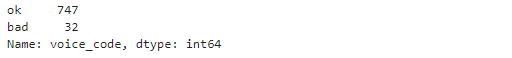
\includegraphics{img/VoiceCodeBefore.png}
	\end{figure}

	And after applying the function to the original data set we ended up with a total of 717 instances after deleting the 32 with value "bad" for the attribute "voice\_code".
	
	In addition of the previous, in order to further clean the data I will proceed by deleting any instances that have an undefined value for any of the attributes. Although in some scenarios those could be considered a valid value for some attributes, given the nature of our features I rather considered them to be failures in the readings. When eliminating the rows with undefined values I did not just limit myself to erasing the ones with an undefined value in one or more of the attributes that would be imputed on the Neuronal Network but rather I eliminated any row with at least one undefined values in any attribute because when considering this to be a failure in the readings I could not trust that the error did not reflect in the values of the other attributes.
	
	This process of deleting the rows with undefined values can be easily done by invoking the dropna method of the pandas dataframe class.
	
	Then, after further analyzing the data I realized that some of the instances had an empty string value for the gender and as I do believe that this could be a significant attribute to input in the neuronal network i decided such value was not valid within this project´s frame and so proceeded with deleting all the instances of data with this value in their sex attribute. In order to do so I implemented he following function:
	
	\vspace{5mm}
	
	\begin{lstlisting}[language=Python]
		
	def eliminateEmptySexElements(data_frame):
		valid_voice_code_elemnts = data_frame.copy()
		valid_voice_code_elemnts = valid_voice_code_elemnts.drop(valid_voice_code_elemnts[valid_voice_code_elemnts["voice_code"] == "" ].index)
		return valid_voice_code_elemnts
	\end{lstlisting}
	
	Finally I also deleted any instances for which the current\_age attribute was lower than the years\_since\_first\_symptom, as such a condition is not logically possible, and also removed all instances with less than 20 as their current\_age value. Which basically eliminated some instances that had a value of 0 for current\_age. I did so with the following function:
	
	\vspace{5mm}
	
	\begin{lstlisting}[language=Python]
		
	def checkAgeIsGraterThanSysptoms(data_frame):
		valid_data_frame = data_frame.copy().reset_index()
		indexes = []
		for index in range(len(valid_data_frame)):
			if valid_data_frame["current_age"][index] < valid_data_frame["years_since_first_symptom"][index] or valid_data_frame["current_age"][index] < 20:
				indexes.append(index)
		valid_data_frame.drop(indexes)
		del valid_data_frame["index"]
		return valid_data_frame
	\end{lstlisting}
	
	\clearpage
	
	\subsection{Normalizing The Data Set And Transforming Non Numerical Values }
	
	Normalizing the data previously to training a Neuronal Network with it bares the benefit of speeding up the learning rates by leading to a faster convergence, this is archived by adjusting the range of values of the different attributes to be the same.\cite{normalization}
	
	In my case I first implemented the min max technique which consists in transforming for every feature it´s minimum value to a zero, it´s maximum value to a one, and then every other value to a decimal between this two.\cite{normalizationTechniques}
	
	\[ x \forall Z \]
	\[ f(x) = (x - MIN(Z))/(MAX(Z)-MIN(Z)) \]
	
	The only significant downside to this technique is the fact that it does not handle outliers well. And according to their plots this would be a problem for several of the features.
	
	We can see the previous problematic represented in the following plot:
	
	\begin{figure}[h]
		\label{Feature02N}
		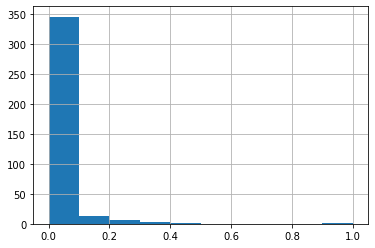
\includegraphics{img/plots/feature02N.png}
		\caption{Histogram for a normalized attribute with outliers. Feature02}
	\end{figure}
	
	In order to minimize the impact of applying the min max technique to those attributes with outliers I decided to apply feature clipping which caps a all features above and below the given boundaries to a fixed value, this on time will help spread the feature values over the entire range. Although this is a helpful technique I did not considered it appropriate for the features which plot shape was similar to the one in Figure 1 and only applied it to some of the attributes with plots that looked similar to the following figure.
	
	\begin{figure}[h]
		\label{Feature24N}
		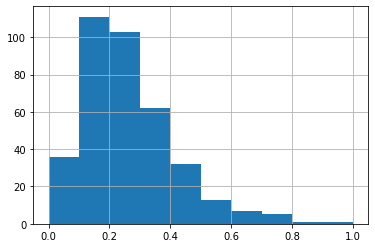
\includegraphics{img/plots/feature24N.png}
		\caption{Histogram for a normalized attribute with outliers. Feature24}
	\end{figure}

	Which after the feature clipping process ended up looking like this:
	
	\begin{figure}[H]
		\label{Feature24NC}
		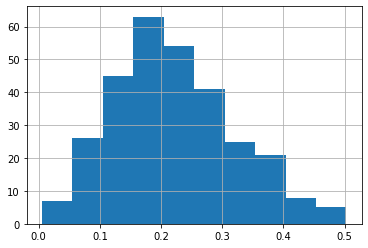
\includegraphics{img/plots/feature24NClip.png}
		\caption{Histogram for a normalized and clipped attribute. Feature24}
	\end{figure}

	In order to archive this improvement in the closeness of the different attributes distributions shapes to a normal distribution I implemented a function based on the Z-Score value of the elements to eliminate any and all outliers of the distribution that showed a relevant degree of skewness whether it is to the right or left.
	
	The formula for the Z-Score is $ Z-Score(x) = (x - \mu)/\sigma $ where $\mu$ stands for the mean and $\sigma$ the standard deviation of the distribution D for which $X \in D$.\cite{datascienceZscore}
	
	\vspace{5mm}
	
	\begin{lstlisting}[language=Python]
		
	def clipZScores(data_frame):
		current_dataframe = data_frame.copy()
		z_scores = zscore(current_dataframe[CLIP_FEATURES])
		abs_z_scores = np.abs(z_scores)
		filtered_entries = (abs_z_scores < 2).all(axis=1)
		new_df = current_dataframe[filtered_entries]
		return new_df
	\end{lstlisting}

	Finally to the several attributes with a value distribution similar to the one presented by "feature02" I thought about applying Log Scaling, which aims to compress a wide range of values into a smaller range and is nice to use when a handful of the values repeat many times as happens for those attributes.\cite{normalizationTechniques}
	
	\[ x \forall Z \]
	\[ f(x) = log(x) \]
	
	It was after my initial attempt that I realized that many of those attributes have features with zero and negative values which actually complicates the application of the Log Scaling and so I decided to try using the RobustScaler and StandardScaler from Python´s sklearn library.
	
	The RobustScaler uses the same formula $f(x) = (x - M)/(Q3-Q1)) $ where M stands for the median and Q1 and Q3 for the first and third quartiles of a distribution D for which $X \in D$.\cite{normalizeSkLearn}
	
	The StandardScaler uses the same formula that was implemented for calculating the Z-Score values in the clipZScores function shown above.
	
	\begin{figure}[H]
		\label{Feature03Comparidson}
		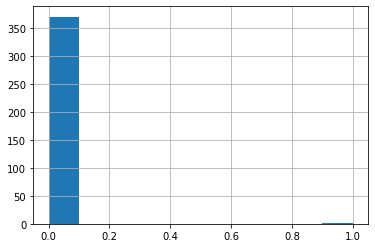
\includegraphics[height=34mm]{img/plots/feature03N.png}
		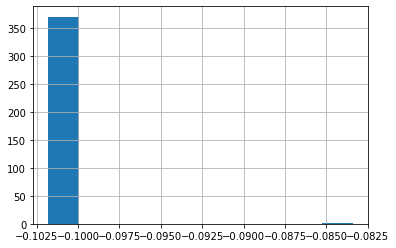
\includegraphics[height=34mm]{img/plots/feature03NStandard.png}
		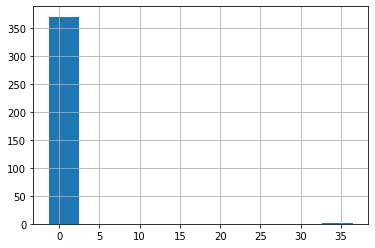
\includegraphics[height=34mm]{img/plots/feature03NRobust.png}
		\caption[width=50mm]{Comparison for normalization applying max min, RobustScaler and StandardScaler. Feature03}
	\end{figure}

	As It can be appreciated in the different plots none of the different techniques got a final distribution closer to a normal than the others and so I decided to simply apply max min to all the attributes.
	
	At this point in time I also assigned numerical values to "sex", which happens to be the only non numerical attribute  that was selected as input for the Neuronal Network. This particular attribute only has two possible values after the cleaning process which are "F" for female participants and "M" for male ones, and so the following function assigns the value 1 for male participants and 0 for female ones.
	
	\vspace{5mm}
	
	\begin{lstlisting}[language=Python]
		
	def normalizeSex(data_frame):
		current_dataframe = data_frame.copy().reset_index()
		n_sex = []
		for index in range(len(current_dataframe)):
			if current_dataframe["sex"][index] == "M":
				n_sex.append(0)
			else:
				n_sex.append(1)
		current_dataframe["sex"] = n_sex
		del current_dataframe["index"]
		return current_dataframe
	\end{lstlisting}
	
	\clearpage
	
	\subsection{Splitting The Data Set}
	
	When working with Neuronal Notworks among other machine learning algorithms it is important to prepare several Data sets for the different activities related to the training of the program and the evaluation of its results. In order to do so it is advisable to split the data in the following three different groups:\cite{dateTestsDefs}
	
	\begin{itemize}
		
		\item \textbf{The training data set:} which includes all the data to which the model will be fitted.
		
		\item \textbf{The validation data set:} which includes all the data to be used as reference for the evaluation of a model fit while fine tuning its hyper parameters. The evaluation of the algorithm over this dataset produces the so called data snooping bias which could make it so your predictions are too optimistic.
		
		\item \textbf{The test data set:} which includes all the data to be used as unbiased reference for the evaluation of an already tuned model fit. The evaluation over this dataset can only be affected by the bias derived from choosing some metrics or the others to evaluate the performance of the algorithm.
		
	\end{itemize}

	The creation and implementation of this three groups in the different stages of the training process has the objective of obtaining a final evaluation of the performance of the algorithm as realistic as possible by avoiding any non realistic outcomes that could come from of the over or under fitting of the model to the training data.
	
	Although our dataset came already divided in two files one for train and one for test both files have approximately the same size, 388 elements on the train file and 390 on the one for test, which did not mach the distribution I was looking for. In order to make sets of the sizes I was aiming for I first combined both files into one dataframe and later created the different sets with the following function that I got from the Hands-On Machine Learning with Scikit-Learn, Keras, and TensorFlow \footnote{The function was originally named split\_train\_test but I decided to rename it to something more fitting to its porpouse within the scope of this project.} \cite{handsonmachinelearning}:
	
		\vspace{5mm}
	
	\begin{lstlisting}[language=Python]
		
	def split_dataset(data, test_ratio):
		shuffled_indices = np.random.permutation(len(data))
		test_set_size = int(len(data) * test_ratio)
		test_indices = shuffled_indices[:test_set_size]
		train_indices = shuffled_indices[test_set_size:]
		return data.iloc[train_indices], data.iloc[test_indices]
	\end{lstlisting}
	
	And so after applying all the steps from the previously described data cleaning process I utilized this function to first divide the dataframe containing all the data into the train and validation data sets with a proportion of 80 to 20 and afterwards divide the train data set into the train and test data sets again with the same proportions.
	
	After all of this I ended up with train, validation and test datasets consisting of 238, 74 and 59 elements respectively.
	
	%No incluir en la memoria. More specifically, you train multiple models with various hyperparameters on the reduced training set (i.e., the full training set minus the validation set), and you select the model that performs best on the validation set. After this holdout validation process, you train the best model on the full training set (including the validation set), and this gives you the final model. Lastly, you evaluate this final model on the test set to get an estimate of the generalization error.
	
	\clearpage
	
	\subsection{Generating The Labels}
	
	The final step was then to generate the labels for each feature and for this I decided to create two separate groups. This first one would encompass all elements with a value for the attribute "years\_since\_first\_symptom" grater than 0 and the second one  would be its complementary. Finally I labeled all the elements within the firsts group with a value of 1 and the others with 0. 
	
	\vspace{5mm}
	
	\begin{lstlisting}[language=Python]
		
	def getDataFrameLabels(data_frame):
		TIENE_PARKINSON = 1
		NO_TIENE_PARKINSON = 0
		data_labels = []
		data_frame.head()
		for elem in data_frame["years_since_first_symptom"]:
			if (elem > 0):
				data_labels.append(TIENE_PARKINSON)
			else:
				data_labels.append(NO_TIENE_PARKINSON)
		return data_labels
	\end{lstlisting}
	
	I applied this process to each of the previously generated train, test and validation data sets individually. 
	
	\clearpage
	
	\section{Implementation of the CNN}
	\label{sec:CNNImplementation}
	
	\clearpage
	
	\subsection{Problems with the algorithm}
	\label{sec:ProblemsWithAlgorithm}
	
	In Machine Learning this is called overfitting: it means that the model performs well on the training data, but it does not generalize well.
	
	Overfitting happens when the model is too complex relative to the amount and noisiness of the training data. Here are possible solutions:
	
	*Simplify the model by selecting one with fewer parameters (e.g., a linear model rather than a high-degree polynomial model), by reducing the number of attributes in the training data, or by constraining the model. (regularization)
	
	Gather more training data.
	
	Reduce the noise in the training data (e.g., fix data errors and remove outliers).
	
	*The amount of regularization to apply during learning can be controlled by a hyperparameter. A hyperparameter is a parameter of a learning algorithm (not of the model). As such, it is not affected by the learning algorithm itself; it must be set prior to training and remains constant during training. If you set the regularization hyperparameter to a very large value, you will get an almost flat model (a slope close to zero); the learning algorithm will almost certainly not overfit the training data, but it will be less likely to find a good solution. Tuning hyperparameters is an important part of building a Machine Learning system (you will see a detailed example in the next chapter).
	
	As you might guess, underfitting is the opposite of overfitting: it occurs when your model is too simple to learn the underlying structure of the data.
	
	Select a more powerful model, with more parameters.
	Feed better features to the learning algorithm (feature engineering).
	Reduce the constraints on the model (e.g., reduce the regularization hyperparameter).
	
	\clearpage
	
	\subsection{Problems with the data}
	
	Insufficient Quantity of Training Data.
	
	Even for very simple problems you typically need thousands of examples, and for complex problems such as image or speech recognition you may need millions of examples.
	
	Nonrepresentative Training Data
	
	In order to generalize well, it is crucial that your training data be representative of the new cases you want to generalize to. This is true whether you use instance-based learning or model-based learning.
	
	It is crucial to use a training set that is representative of the cases you want to generalize to. This is often harder than it sounds: if the sample is too small, you will have sampling noise (i.e., nonrepresentative data as a result of chance), but even very large samples can be nonrepresentative if the sampling method is flawed. This is called sampling bias.
	
	Poor-Quality Data %debería considerarlo ? 
	Synapse tiene un control de calidad, columna que categoriza el audio en correcto o no 
	
	Irrelevant Features
	As the saying goes: garbage in, garbage out. Your system will only be capable of learning if the training data contains enough relevant features and not too many irrelevant ones. A critical part of the success of a Machine Learning project is coming up with a good set of features to train on. This process, called feature engineering, involves the following steps:
	
	Feature selection (selecting the most useful features to train on among existing features)*
	
	Feature extraction (combining existing features to produce a more useful one as we saw earlier, dimensionality reduction algorithms can help)
	
	Creating new features by gathering new data
	
	*Visualization algorithms are also good examples of unsupervised learning
	
	A related task is dimensionality reduction, in which the goal is to simplify the data without losing too much information. One way to do this is to merge several correlated features into one. For example, a car’s mileage may be strongly correlated with its age, so the dimensionality reduction algorithm will merge them into one feature that represents the car’s wear and tear. This is called feature extraction.
	
	\clearpage
	
	\subsubsection{Balancing The Data Set}
	
	
	
	\clearpage
	
	\section{Conclusions}
	
	\clearpage
	
	\subsection{Possible Future Work Lines}
	
	Yet another important unsupervised task is anomaly detection—for example, detecting unusual credit card transactions to prevent fraud, catching manufacturing defects, or automatically removing outliers from a dataset before feeding it to another learning algorithm. The system is shown mostly normal instances during training, so it learns to recognize them; then, when it sees a new instance, it can tell whether it looks like a normal one or whether it is likely an anomaly
	
	\clearpage
	
	\subsection{Social Implications}
	
	
	\clearpage
	
	
	
	\bibliography{bibliografia.bib}
	
	\bibliographystyle{IEEEtran}
	
\end{document}




